%!TeX root=./par.tex

\FloatBarrier


\section{Algoritmo estático}\label{sec:algoritmo-estatico}

O algoritmo que será aqui apresentado foi proposto por Basch, Guibas
e Hershberger [\cite{BASCH19991}] e admite uma boa cinetização, usando a ideia de linha
de varredura.

O algoritmo é baseado na ideia de dividir o plano, para cada ponto, em seis cones iguais.
Os cones são delimitados pela reta paralela ao eixo $y$ que passa pelo ponto e pelas retas $x \pm
30^\circ$, isto é, as retas que passam pelo ponto e formam $\pm 30^\circ$ com o eixo $x$ como mostra a
Figura~\ref{fig:parestatico:cones}.

\begin{figure}
    \centering
    \begin{tikzpicture}[thick]
        \draw (0, -3) -- (0, 3) node[anchor=north west] {$y$};
        \draw (-3, 1.7302) -- (3, -1.7302)
            node[anchor=north west] {$x - 30^\circ$};
        \draw (-3, -1.7302) -- (3, 1.7302)
            node[anchor=south west] {$x + 30^\circ$};
        \node[label=250:$p$] (p) at (0, 0) {\textbullet};
    \end{tikzpicture}
    \caption[Exemplo de cones do algoritmo estático]{A reta paralela
    ao eixo $y$ que passa por $p$ e as retas $x \pm 30^\circ$.}
    \label{fig:parestatico:cones}
\end{figure}

Tendo dividido o plano em cones, a ideia é achar o ponto mais próximo de $p$ dentro de cada um
desses cones.
Se assim o fizermos para todos os pontos, um desses pares possui a menor distância entre si e será
um par mais próximo que buscamos.

Se $(p, q)$ formam um par mais próximo, então $(q, p)$ também forma um par mais próximo;
na verdade, são o mesmo par.
Dessa maneira, não precisamos dos seis cones para buscar os pares, somente de três deles.
Para uma varredura da direita para a esquerda, apenas buscaremos os pares mais próximos nos três
cones à direita de p.

Vamos começar analisando o cone cujo eixo central é paralelo ao eixo $x$.
Chamaremos esse cone de \textit{dominância de p} e o representaremos por $\Dom(p)$.
Consideraremos que um ponto em cima da linha $x + 30^\circ$ pertence a $\Dom(p)$ e um ponto em cima de
$x - 30^\circ$ não pertence a $\Dom(p)$ como mostra a Figura~\ref{fig:parestatico:dominancia}.
O mesmo algoritmo poderá ser aplicado aos outros dois cones se rotacionarmos o sistema de
coordenadas~$\pm 60^\circ$.

\begin{figure}[H]
    \centering
    \begin{tikzpicture}[thick, scale=0.8]
        % \draw (0, -3) -- (0, 3) node[anchor=north west] {$y$};
        \draw (0, 0) -- (4, 2.309);
        \draw[dashed] (0, 0) -- (4, -2.309);
        \draw (0, 0) circle (2pt) node[label=250:$p$] {};
        \node[label=0:$q$] (q) at (1, 0) {\textbullet};
        \node[label=250:$r$] (r) at (3, 1.715) {\textbullet};
        \draw (3, -1.73) circle (2pt) node[label=250:$s$] {};
        % \node[label=250:$s$] (s) at (3, -1.73);
    \end{tikzpicture}
    \caption[Exemplo de $\Dom(p)$]{Os pontos $q$ e $r$ pertencem a $\Dom(p)$,
    mas os pontos $p$ e $s$ não.}
    \label{fig:parestatico:dominancia}
\end{figure}

A Figura~\ref{fig:parestatico:conjuntos}, inspirada em~\cite{BASCH19991}, ilustra cada uma das
definições a seguir.
Definiremos como $\Maxima(p)$ o conjunto dos pontos à direita de $p$ que não pertencem à
dominância de nenhum ponto à direita de $p$.
Isso nos permite definir o conjunto de \textit{candidatos} de $p$ representado por $\Cands(p)$:
$\Cands(p) = \Dom(p) \cap\Maxima(p)$, ou seja, os candidatos de $p$ são aqueles pontos à
direita de $p$ que não pertencem à dominância de nenhum ponto à direita de $p$ e
pertencem à dominância de $p$.
Chamaremos o ponto de $\Maxima$ de menor ordenada que está acima de $\Dom(p)$ de $\up(p)$ e
chamaremos o ponto de $\Maxima$ de maior ordenada que está abaixo de $\Dom(p)$ de $\low(p)$.
Caso não existam tais pontos, $\up(p)$ e $\low(p)$ são \nnull.
Os pontos de $\Maxima$ estritamente entre $\low(p)$ e $\up(p)$ são justamente os de $\Cands(p)$.
Dentre os candidatos de $p$, chamaremos o ponto com menor coordenada $x$ de $\lcand(p)$.

\begin{figure}
    \centering
    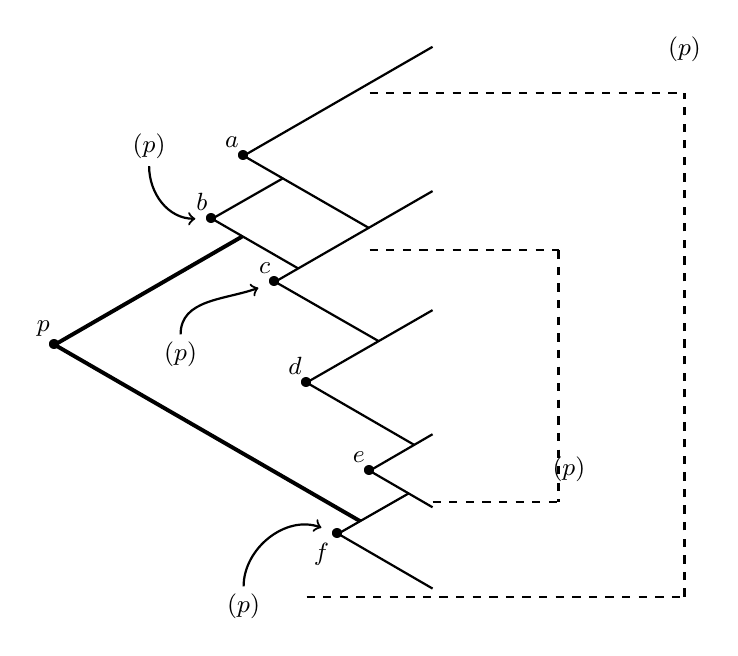
\begin{tikzpicture}[thick, scale=0.8]
        \node[label={[label distance = -3mm]160:$p$}]
            at (0.00, 0.00) {\textbullet};
        \node[label={[label distance = -3mm]160:$a$}]
            (a) at (3.00, 3.00) {\textbullet};
        \node[label={[label distance = -3mm]160:$b$}]
            (b) at (2.50, 2.00) {\textbullet};
        \node[label={[label distance = -3mm]160:$c$}]
            (c) at (3.50, 1.00) {\textbullet};
        \node[label={[label distance = -3mm]160:$d$}]
            at (4.00, -0.60) {\textbullet};
        \node[label={[label distance = -3mm]160:$e$}]
            at (5.00, -2.00) {\textbullet};
        \node[label={[label distance = -3mm]220:$f$}]
            (f) at (4.50, -3.00) {\textbullet};

        % e cone
        \draw (5.00, -2.00) -- (6.00, -2.58);
        \draw (5.00, -2.00) -- (6.00, -1.42);
        % f cone
        \draw (4.50, -3.00) -- (6.00, -3.87);
        \draw (4.50, -3.00) -- (5.62, -2.36);
        % d cone
        \draw (4.00, -0.60) -- (5.71, -1.59);
        \draw (4.00, -0.60) -- (6.00, 0.55);
        % c cone
        \draw (3.50, 1.00) -- (5.14, 0.06);
        \draw (3.50, 1.00) -- (6.00, 2.44);
        % a cone
        \draw (3.00, 3.00) -- (4.98, 1.86);
        \draw (3.00, 3.00) -- (6.00, 4.73);
        % b cone
        \draw (2.50, 2.00) -- (3.87, 1.21);
        \draw (2.50, 2.00) -- (3.62, 2.64);
        % p cone
        \draw[line width = 0.5mm] (0.00, 0.00) -- (4.85, -2.80);
        \draw[line width = 0.5mm] (0.00, 0.00) -- (2.98, 1.72);

        \draw[dashed] (6,-2.5) -- (8, -2.5)
            node[anchor=west, label=90:$\Cands(p)$] {};
        \draw[dashed] (8, 1.5) -- (8, -2.5);
        \draw[dashed] (5,1.5) -- (8, 1.5);

        \draw[dashed] (4, -4) -- (10, -4);
        \draw[dashed] (10, -4) -- (10, 4);
        \draw[dashed] (5, 4) -- (10, 4)
            node[anchor=south, label=$\Maxima(p)$] {};

        \node[label={[label distance = -3mm]270:$\low(p)$}]
            (low) at (3, -4) {};
        \draw[->] (low) edge[out=90,in=160] (f);

        \node[label={[label distance = -3mm]270:$\lcand(p)$}]
            (lc) at (2, 0) {};
        \draw[->] (lc) edge[out=90,in=200] (c);

        \node[label={[label distance = -3mm]90:$\up(p)$}]
            (up) at (1.5, 3) {};
        \draw[->] (up) edge[out=270,in=180] (b);
    \end{tikzpicture}
    \caption{Os pontos $c$, $d$ e $e$ pertencem a $\Cands(p)$, e todos os
    pontos exceto $p$ pertencem a $\Maxima(p)$. O ponto $b$ é $\up(p)$ e o
    ponto $f$ é $\low(p)$. O ponto $c$ é $\lcand(p)$.}
    \label{fig:parestatico:conjuntos}
\end{figure}

Consideraremos apenas os pares $(p, \lcand(p))$ como possíveis candidatos a par mais próximo.
Caso, para algum $p$, mais de um ponto atenda à condição de ser $\lcand(p)$ poderemos escolher
qualquer um deles como $\lcand(p)$, pois, em um caso em que há mais de um possível $\lcand(p)$,
esses pontos formarão um par mais próximo entre si do que o par $(p, \lcand(p))$, como por exemplo
na Figura~\ref{fig:parestatico:lcands}.

\begin{figure}
    \centering
    \begin{tikzpicture}[thick]
        % \draw (0, -3) -- (0, 3) node[anchor=north west] {$y$};
        \draw (0, 0) -- (4, 2.309);
        \draw[dashed] (0, 0) -- (4, -2.309);
        \node[label=250:$p$] (p) at (0, 0) {\textbullet};
        \node[label=0:$q$] (q) at (4, -1) {\textbullet};
        \node[label=250:$r$] (r) at (4, 1) {\textbullet};
        \draw[dotted] (4, -1) -- (4, 1);
        \draw[dotted] (0, 0) -- (r);
        \draw[dotted] (0, 0) -- (q);
    \end{tikzpicture}
    \caption{A distância de $r$ até $q$ é menor do que a
    distância $p$ até $r$ e do que a distância $p$ até $q$.}
    \label{fig:parestatico:lcands}
\end{figure}

O Algoritmo~\ref{alg:par-estatico:horizontal} descreve a sequência de operações a serem feitas para
achar o par mais próximo em alguma das ordens $(-60^\circ, 0^\circ, 60^\circ)$ representadas pelo
ângulo $\theta$, dado em radianos.
Antes da rotina ser chamada, os pontos devem ser ordenados de acordo com a sua coordenada $x$.
Os pontos são então processados da direita para a esquerda.
No algoritmo, $a$ e $b$ são os pontos que representam o par mais próximo.
Se $p$ ou $q$ são nulos, $d(p,q)$ retorna $+\infty$.

A cada iteração do Algoritmo~\ref{alg:par-estatico:horizontal}, $\Maxima$ é igual a $\Maxima(p)$.
Na nossa implementação, $\Maxima$ estará armazenado em uma árvore binária de busca, mais
especificamente em uma \textit{splay tree} cuja chave é a coordenada $y$ dos pontos, determinada
de acordo com o valor de $\theta$.
Com isso, podemos buscar por $\up(p)$ e $\low(p)$ em tempo logarítmico, bem como podemos retirar
$\Cands(p)$ de $\Maxima$ em tempo logarítmico, isto é, atualizar $\Maxima$ de maneira que $\Maxima
= \Maxima \setminus \Cands(p)$.

\begin{algorithm}
    \caption[Algoritmo \textsc{closest\_pair} do par mais próximo]{Função \textsc{closest\_pair}$(p, n, \theta)$.}
    \label{alg:par-estatico:horizontal}
    \begin{algorithmic}[1]
        \Function{closest\_pair}{$p, n, \theta$}
            \State \Call{heapsort}{$p, n, \theta$} \Comment{$p[1].x > \cdots > p[n].x$}
            \State $(a,b) \leftarrow (\nnull, \nnull)$
            \State $\Maxima \leftarrow \varnothing$
            \For{$i \leftarrow 1\To n$}
                \State $\Cands \leftarrow \Maxima\cap \Dom(p[i])$
                \State $\Maxima \leftarrow (\Maxima \setminus \Cands) \cup \lk p[i]\rk$
                \State $\lcand \leftarrow \Call{min\_x}{\Cands}$
                \If{$d(p[i], \lcand) < d(a, b)$}
                    \State $(a, b) \leftarrow (p[i], \lcand)$
                \EndIf
            \EndFor
            \State \Return{$(a, b)$}
        \EndFunction
    \end{algorithmic}
\end{algorithm}

Para descrever a implementação do algoritmo, já considerando as versões rotacionadas dele, iremos
antes precisar estabelecer os nomes das variáveis e rotinas auxiliares utilizadas.
São elas:
\begin{enumerate}
    \item $n$: o número de pontos dados;
    \item \textit{point}: um ponto com os seguintes atributos:
    \begin{enumerate}
        \item $x$: coordenada $x$ do ponto;
        \item $y$: coordenada $y$ do ponto.
    \end{enumerate}
    \item \raiz: raiz da splay tree;
    \item \no: objeto que compõe a árvore binária de busca,
    atributos:
    \begin{enumerate}
        \item \esq$:$ aponta para a raiz da subárvore esquerda do nó.
        A subárvore esquerda é composta apenas por pontos que possuem
        \textit{value}~com menor ordenada que a \textit{value}~do nó;
        \item \dir$:$ aponta para a raiz da subárvore direita do nó.
        A subárvore direita é composta apenas por pontos que possuem
        \textit{value}~com ordenada maior ou igual que a \textit{value}~do nó;
        \item \pai$:$ aponta para o nó que é pai deste nó;
        \item \textit{value}$:$ aponta para um ponto.
    \end{enumerate}
    \item \angulo: ângulo de rotação do sistema de coordenadas;
    \item \pontos: vetor de $n$ posições que guarda os pontos;
    \item \textsc{getX}$(p, \angulo) \rightarrow$ retorna a coordenada $x$
    de um ponto $p$ baseada no ângulo de rotação \angulo;
    \item \textsc{getY}$(p, \angulo) \rightarrow$ retorna a coordenada $y$
    de um ponto $p$ baseada no ângulo de rotação \angulo;
    \item \textsc{heapsort}$(\pontos, n, \angulo) \rightarrow$ ordena o vetor \pontos,
    utilizando o algoritmo \textit{heapsort}, de acordo com a coordenada $x$ de cada ponto cujo
    valor é retornado pela rotina \textsc{getX}$(p, \angulo)$.
\end{enumerate}

Para um ponto $(r, \phi)$ em coordenadas polares, $x = r\cdot \cos{(\phi)}$ e $y = r\cdot
\sin{(\phi)}$.

Rotacionar o sistema de coordenadas por $\theta$ é o mesmo que transformar $\phi$ em $\phi -
\theta$, veja a Figura~\ref{fig:parestatico:rotacao}.
Isso significa que agora as novas coordenadas são descritas como:
\begin{align*}
    x^* & = r\cdot \cos{(\phi - \theta)}= r\cdot \cos{(\phi)}\cdot \cos{(\theta)}
    + r\cdot \sin{(\phi)}\cdot \sin{(\theta)} = x\cdot \cos{(\theta)} + y\cdot \sin{(\theta)} \\
    y^* & = r\cdot \sin{(\phi - \theta)} = r\cdot \sin{(\phi)}\cdot \cos{(\theta)}
    - r\cdot \cos{(\phi)}\cdot \sin{(\theta)} = y\cdot \cos{(\theta)} - x\cdot \sin{(\theta)}.
\end{align*}
Os valores $x^*$ e $y^*$ são os valores, respectivamente, retornados por \textsc{getX}$(p,
\angulo)$ e \textsc{getY}$(p, \angulo)$ para $\theta = \angulo$.

\begin{figure}[H]
    \centering
    \begin{tikzpicture}[thick,scale=0.8]
        \coordinate (a) at (0, 0);
        \coordinate (b) at (4, 0);
        \coordinate (c) at (2.828, 2.828);
        \coordinate (p) at (1, 2);
        \draw[thick,->] (0,0) -- (4,0)
        node[anchor=north west] {$x$};
        \draw[thick,->] (0,0) -- (0,4)
        node[anchor=south east] {$y$};
        \draw[thick,->, dashed] (0,0) -- (2.828,2.828)
        node[anchor=north west] {$x'$};
        \draw[thick,->, dashed] (0,0) -- (-2.828,2.828)
        node[anchor=south east] {$y'$};
        \pic [draw, angle radius = 0.5cm] {angle = b--a--c};
        \node[anchor=west, label={[label distance = 0mm]180:$\theta$}]
        (angl) at (1, 0.3) {};
        \node[label=90:$p$] at (p) {\textbullet};
        \draw[dashed,->] (a) -- node[above] {$r$} (p);
        \pic [draw, angle radius = 1cm] {angle = b--a--p};
        \node[anchor=west, label={[label distance = -3mm]180:$\phi$}]
        (angp) at (1.2, 0.7) {};
    \end{tikzpicture}
    \caption[Exemplo de rotação dos pontos]{O ponto $p$ está numa inclinação de $\phi - \theta$ radianos
    em relação a reta que passa pela origem e por $x'$.}
    \label{fig:parestatico:rotacao}
\end{figure}

A interface da \textit{splay tree} que vai armazenar $\Maxima$, e cuja chave é a coordenada $y$ do
ponto, contará com as seguintes operações, além das usuais \textsc{insert}$(p)$ e
\textsc{splay}$(x)$:
\begin{enumerate}
    \item \textsc{successor}$(p) \rightarrow$ busca pelo nó
    cuja chave é $\up(p)$ na \textit{splay tree}.
    Esse nó corresponde ao sucessor de $p$ na árvore;
    \item \textsc{predecessor}$(p) \rightarrow$ busca pelo nó cuja chave é $low(p)$ na \textit{splay tree}.
    Esse nó corresponde ao predecessor de $p$ na árvore;
    % \item \textsc{splay}$(x) \rightarrow$ dá um \textit{splay} no nó $x$;
    \item \textsc{lcand}$(p) \rightarrow$ calcula $\Cands(p)$, remove da
    \textit{splay tree} e determina $\lcand(p)$, que pode ser \nnull;
    % \item \textsc{clearAll}$() \rightarrow$ remove todos os nós
    % da \textit{splay tree}.
\end{enumerate}

% As operações \textsc{insert}$(p)$, \textsc{splay}$(x)$ e
% \textsc{clearAll}$()$ não possuem nenhuma diferença quanto
% à sua implementação. São operações comuns de uma
% \textit{splay tree}. Portanto, focaremos em explicar as
% operações successor$(p)$, predecessor$(p)$ e lcand$(p)$.

No Algoritmo~\ref{alg:par-estatico:successor} e no Algoritmo~\ref{alg:par-estatico:predecessor}, a rotina
\textsc{checkLine}$(p, q, \theta)$ retorna se o ponto$q$ está à esquerda, sobre ou à direita da
reta $r$.
A reta $r$ é a reta que passa por $p$ e faz um ângulo de $\theta$ radianos com o eixo $x$.
Para $q$ à esquerda de $r$ o retorno é $1$, para $q$ sobre $r$ o retorno é $0$ e para $q$ à
direita de $r$, o retorno é $-1$.

O Algoritmo~\ref{alg:par-estatico:lcand} implementa a função \textsc{lcand}$(p)$.
Sabemos que $\lcand(p)$ é o elemento de $\Cands(p)$ com menor coordenada $x$ e que $\Cands(p)$ é
limitado por $\low(p)$ e $\up(p)$.
A ideia para retirar $\Cands(p)$ da árvore é reorganizá-la de modo que $\low(p)$ seja a raiz e
$\up(p)$ o filho direito da raiz.
Dessa forma $\Cands(p)$ é a subárvore esquerda do filho direito da raiz, veja a
Figura~\ref{fig:parestatico:loweup}.
Nem sempre tal configuração é possível, mas o algoritmo tratará dos casos de borda que são quando
$\low(p)$, ou $\up(p)$, ou ambos, não existem.
A rotina \textsc{split}$(x)$ separa a subárvore de raiz $x$ da \textit{splay tree} e retorna a
raiz dessa nova árvore.
A rotina \textsc{min\_x}$(z)$ retorna o ponto com menor coordenada $x$ da árvore de raiz~$z$.

\begin{figure}[H]
    \centering
    \begin{tikzpicture}[thick]
        \tikzstyle{every node}=[font=\small]
        \node[every node,circle,draw, minimum size=1cm] (low) at (0, 0) {$l$};
        \node[every node,circle,draw, minimum size=1cm] (up) at (2, -2) {$u$};
        \node (esq) at (-2, -2) {$\gamma$};
        \node[every node] (esqesq) at (1, -4) {$\alpha$};
        \node[every node] (esqdir) at (3, -4) {$\beta$};
        \draw (low) -- (up);
        \draw (esqesq) -- (up);
        \draw (esqdir) -- (up);
        \draw (low) -- (esq);
    \end{tikzpicture}
    \caption{Se $l$ é $\low(p)$ e $u$ é $\up(p)$. A subárvore
        $\alpha$ contém todos os pontos que estão entre $\low(p)$ e
        $\up(p)$ e, portanto, corresponde ao conjunto $\Cands(p)$.}
    \label{fig:parestatico:loweup}
\end{figure}

\begin{algorithm}
    \caption{Função \textsc{successor}$(p)$.}
    \label{parestatico:successor}
\begin{algorithmic}[1]
    \Function{successor}{$p$}
        \State $x \leftarrow \raiz$
        \State $up \leftarrow NULL$
        \While{$x \neq NULL$}
            \State $y \leftarrow x$
            \If{$\Call{checkLine}{p, x.key, \pi/6}= -1$}
                \State $x \leftarrow x.right$
            \Else
                \State $up \leftarrow x$
                \State $x \leftarrow x.left$
            \EndIf
        \EndWhile
        \If{$y \neq NULL$} \Comment{dá \textsc{splay} no último nó visitado}
            \State \Call{splay}{$y$}
        \EndIf
        \State \Return{$up$}
    \EndFunction
\end{algorithmic}
\end{algorithm}

\begin{algorithm}
    \caption{Função \textsc{predecessor}$(p)$.}
    \label{parestatico:predecessor}
\begin{algorithmic}[1]
    \Function{predecessor}{$p$}
        \State $x \leftarrow \raiz$
        \State $low \leftarrow NULL$
        \While{$x \neq NULL$}
            \State $y \leftarrow x$
            \If{$\Call{checkLine}{p, x.key, -\pi/6}\leq 0$}
                \State $x \leftarrow x.left$
            \Else
                \State $low \leftarrow x$
                \State $x \leftarrow x.right$
            \EndIf
        \EndWhile
        \If{$y \neq NULL$} \Comment{dá \textsc{splay} no último nó visitado}
            \State \Call{splay}{$y$}
        \EndIf
        \State \Return{$low$}
    \EndFunction
\end{algorithmic}
\end{algorithm}

\begin{algorithm}
    \caption{Função lcand$(p)$.} \label{parestatico:lcand}
    \begin{algorithmic}[1]
        \Function{lcand}{$p$}
            \State $r \leftarrow \raiz$
            \State $\low \leftarrow \Call{predecessor}{p}$
            \If{$\low \neq \nnull$}
                \State \Call{splay}{$\low$}
                \State $r \leftarrow \Call{split}{\low.\dir}$
            \EndIf
            \State $\up \leftarrow \Call{successor}{p}$
            \If{$\up \neq \nnull$}
                \State $\Call{splay}{\up}$
                \State $r \leftarrow \Call{split}{\up.\esq}$
            \EndIf
            \If{$\up \neq \nnull$ \AND $\low \neq \nnull$}
                \State $\low.\dir \leftarrow \up$
                \State $\up.\parent \leftarrow \low$
            \EndIf
            \State \Return{\Call{min\_x}{$r$}}
        \EndFunction
    \end{algorithmic}
\end{algorithm}

O Algoritmo~\ref{alg:par-estatico:closest} implementa a função \textsc{query\_closest} que retorna um
par $(a,b)$ que possui distância mínima em \pontos.

\begin{algorithm}[H]
    \caption[Algoritmo \textsc{query\_closest} do par mais próximo]{Função \textsc{query\_closest}.} \label{alg:par-estatico:closest}
    \begin{algorithmic}[1]
        \Function{query\_closest}{\null}
            \State $(m,n) \leftarrow (\nnull, \nnull)$
            \State \angulo~$\leftarrow -\frac{\pi}{3}$
            \While{\angulo~$\leq \frac{\pi}{3}$}
                \State \Call{heapsort}{$\pontos, n, \angulo$} \Comment{$\pontos.x[1] > \cdots >
                \pontos.x[n]$}
                \For{$i \leftarrow 1$\To$n$}
                    \State $p \leftarrow $~\pontos$[i]$
                    \State $\lcand \leftarrow $ \Call{lcand}{$p$}
                    \State \Call{insert}{$p$}
                    \If{$d(p, \lcand) < d(a, b)$}
                        \State $(a, b) \leftarrow (p, \lcand)$
                    \EndIf
                \EndFor
                \State \angulo~$\leftarrow$~\angulo~$ + \frac{\pi}{3}$
                \State \Call{clearAll}{\null} \Comment{esvazia a \textit{splay tree}}
            \EndWhile
            \State \Return{$(m,n)$}
        \EndFunction
    \end{algorithmic}
\end{algorithm}
